%%%%%%%%%%%%%%%%%%%%%%%%%%%%%%%%%%%%%%%%%
% Beamer Presentation
% LaTeX Template
% Version 1.0 (10/11/12)
%
% This template has been downloaded from:
% http://www.LaTeXTemplates.com
%
% License:
% CC BY-NC-SA 3.0 (http://creativecommons.org/licenses/by-nc-sa/3.0/)
%
%%%%%%%%%%%%%%%%%%%%%%%%%%%%%%%%%%%%%%%%%

%----------------------------------------------------------------------------------------
%	PACKAGES AND THEMES
%----------------------------------------------------------------------------------------

\documentclass[10pt]{beamer}


\mode<presentation> {
	
	% The Beamer class comes with a number of default slide themes
	% which change the colors and layouts of slides. Below this is a list
	% of all the themes, uncomment each in turn to see what they look like.
	
	%\usetheme{default}
	%\usetheme{AnnArbor}
	%\usetheme{Antibes}
	%\usetheme{Bergen}
	\usetheme{Berkeley}
	%\usetheme{Berlin}
	%\usetheme{Boadilla}
	%\usetheme{CambridgeUS}
	%\usetheme{Copenhagen}
	%\usetheme{Darmstadt}
	%\usetheme{Dresden}
	%\usetheme{Frankfurt}
	%\usetheme{Goettingen}
	%\usetheme{Hannover}
	%\usetheme{Ilmenau}
	%\usetheme{JuanLesPins}
	%\usetheme{Luebeck}
	%\usetheme{Madrid}
	%\usetheme{Malmoe}
	%\usetheme{Marburg}
	%\usetheme{Montpellier}
	%\usetheme{PaloAlto}
	%\usetheme{Pittsburgh}
	%\usetheme{Rochester}
	%\usetheme{Singapore}
	%\usetheme{Szeged}
	%\usetheme{Warsaw}
	
	% As well as themes, the Beamer class has a number of color themes
	% for any slide theme. Uncomment each of these in turn to see how it
	% changes the colors of your current slide theme.
	
	%\usecolortheme{albatross}
	%\usecolortheme{beaver}
	%\usecolortheme{beetle}
	%\usecolortheme{crane}
	%\usecolortheme{dolphin}
	%\usecolortheme{dove}
	%\usecolortheme{fly}
	%\usecolortheme{lily}
	%\usecolortheme{orchid}
	%\usecolortheme{rose}
	%\usecolortheme{seagull}
	\usecolortheme{seahorse}
	%\usecolortheme{whale}
	%\usecolortheme{wolverine}
	
	%\setbeamertemplate{footline} % To remove the footer line in all slides uncomment this line
	%\setbeamertemplate{footline}[page number] % To replace the footer line in all slides with a simple slide count uncomment this line
	
	%\setbeamertemplate{navigation symbols}{} % To remove the navigation symbols from the bottom of all slides uncomment this line
}

\usepackage{amsmath,amssymb}
\usepackage{bm}
\usepackage{copyrightbox}
\usepackage{listings}
\usepackage{array}
\usepackage{tikz}
\usepackage{adjustbox}
\usepackage{ragged2e}
\usepackage{etoolbox}
\usepackage{subfigure}


\usepackage{graphicx} % Allows including images
\usepackage{booktabs} % Allows the use of \toprule, \midrule and \bottomrule in tables
\usepackage{fontawesome5}
\usepackage{url}
\usepackage{hyperref}

\usepackage{bibentry}
%\usepackage[backend=biber,style=ieee, citestyle=authoryear]{biblatex}
%\usepackage[style=ieee-alphabetic, backend=bibtex]{biblatex}
\usepackage[style=numeric, backend=bibtex]{biblatex}



%\bibliography{bibfile.bib}
\addbibresource{assets/bibfile.bib}



\makeatletter
\newcommand*{\mkblankfootnote}[1]{%
	\begingroup
	\renewcommand\thefootnote{}%
	\footnotetext{\bibfootnotewrapper{#1}}%
	\endgroup
}

\newcommand*{\mkbibsupercite}[1]{%
	\def\cbx@savedcites{\cbx@footfullcite}%
	\mkbibbrackets{#1}%
	\ifx\cbx@savedkeys\@empty
	\else
	\cbx@savedcites
	\fi}

\DeclareCiteCommand{\supercite}[\mkbibsupercite]
{\gdef\cbx@savedkeys{}}
{\usebibmacro{citeindex}%
	\usebibmacro{cite}%
	{}%
	\xappto\cbx@savedkeys{\thefield{entrykey},}}
{\supercitedelim}
{\protected@xappto\cbx@savedcites{%
		[\thefield{prenote}][\thefield{postnote}]{\cbx@savedkeys}}}

\DeclareCiteCommand{\cbx@footfullcite}
{}
{\mkblankfootnote{%
		\printtext[labelalphawidth]{%
			\usebibmacro{cite}%
		}%
		\setunit{\addspace}%
		\usedriver
		{\DeclareNameAlias{sortname}{default}}
		{\thefield{entrytype}}}}
{}
{}
\makeatother

\renewcommand*{\nameyeardelim}{\addcomma\addspace}

\apptocmd{\frame}{}{\justifying}{} % Allow optional arguments after frame.

\let\olditem\item
\renewcommand\item{\olditem\justifying}

\addtobeamertemplate{navigation symbols}{}{%
	\usebeamerfont{footline}%
	\usebeamercolor[fg]{footline}%
	\hspace{1em}%
	\insertframenumber/\inserttotalframenumber
}


\makeatletter
\@addtoreset{subfigure}{figure}
\makeatother



\makeatletter
\let\old@lstKV@SwitchCases\lstKV@SwitchCases
\def\lstKV@SwitchCases#1#2#3{}
\makeatother
\usepackage{lstlinebgrd}
\makeatletter
\let\lstKV@SwitchCases\old@lstKV@SwitchCases

\lst@Key{numbers}{none}{%
	\def\lst@PlaceNumber{\lst@linebgrd}%
	\lstKV@SwitchCases{#1}%
	{none:\\%
		left:\def\lst@PlaceNumber{\llap{\normalfont
				\lst@numberstyle{\thelstnumber}\kern\lst@numbersep}\lst@linebgrd}\\%
		right:\def\lst@PlaceNumber{\rlap{\normalfont
				\kern\linewidth \kern\lst@numbersep
				\lst@numberstyle{\thelstnumber}}\lst@linebgrd}%
	}{\PackageError{Listings}{Numbers #1 unknown}\@ehc}}
\makeatother
\newcounter{subListing}[subfigure]

\definecolor{codegreen}{rgb}{0,0.6,0}
\definecolor{codegray}{rgb}{0.5,0.5,0.5}
\definecolor{codepurple}{rgb}{0.58,0,0.82}
\definecolor{mygreen}{RGB}{28,172,0} 
\definecolor{mylilas}{RGB}{170,55,241}
\definecolor{backcolour}{rgb}{1,1,0.98}

\lstset{language=Python,%
	backgroundcolor=\color{backcolour},   
	commentstyle=\color{codegreen},
	keywordstyle=\color{blue},
	numberstyle=\tiny\color{codegray},
	stringstyle=\color{codepurple},
	basicstyle=\tt\scriptsize,
	frame = LBtr,
	%frameround=T,
	rulecolor=\color{gray},
	showstringspaces=false,
	numbers=left,%
	numberstyle={\tiny\color{gray}},
	numbersep=8pt,
	breaklines=true,
	%postbreak=\mbox{\textcolor{yellow}{$\hookrightarrow$}\space},
	tabsize=2,
	escapechar=`,
	xleftmargin=1.8 em, 
	framexleftmargin=2em,
}


%----------------------------------------------------------------------------------------
%	TITLE PAGE
%----------------------------------------------------------------------------------------

\definecolor{AtherosPrimary}{rgb}{0.992156,0.380392,0.34509803921}
\definecolor{AtherosSecondary}{rgb}{0.019,0,0.1568} % UBC Blue (primary)
\definecolor{AtherosTertiary}{rgb}{0.215,0.0625,0.515625}

\setbeamercolor{palette primary}{bg=AtherosSecondary,fg=white}
\setbeamercolor{palette tertiary}{bg=AtherosPrimary,fg=white}
\setbeamercolor{palette secondary}{bg=AtherosTertiary,fg=white}

\title{Advanced Python Programming Workshop} % The short title appears at the bottom of every slide, the full title is only on the title page

\logo{
\includegraphics[width=1.2cm]{assets/logo}}


\author{Mohammad Raziei} % Your name
\institute[Sharif University] % Your institution as it will appear on the bottom of every slide, may be shorthand to save space
{
	\faUniregistry\ Sharif University of Technology\\ % Your institution for the title page
	\medskip
	\href{mailto://mohammadraziei1375@gmail.com}{\faMailBulk\  mohammadraziei1375@gmail.com}\\ % Your email address
	\medskip
	\href{https://github.com/mohammadraziei}{\faGithub\ mohammadraziei} % Your email address
}
\date{\today} % Date, can be changed to a custom date

\graphicspath {{assets/}}

\newcommand{\mypause}{\pause}

\begin{document}
	
	
	% Slide 1: Title Slide
	\begin{frame}
		\titlepage
	\end{frame}
	
	
	\begin{frame}[allowframebreaks]
		\tableofcontents
	\end{frame}
	
	\section{Introduction to Python}
	\subsection{Advantages and Disadvantages of Python}
	\begin{frame}{Advantages and Disadvantages of Python}
		\textbf{Advantages} 
		\hfill \raisebox{-.5cm}{
\includegraphics[width=1cm]{like}} \\[0.1cm]
		\begin{itemize}
			\item Easy to learn and use
			\item Extensive libraries for data analysis (\texttt{Pandas}, \texttt{NumPy}, \texttt{Matplotlib})
			\item Support for machine learning and AI frameworks (\texttt{scikit-learn}, \texttt{TensorFlow}, \texttt{PyTorch})
			\item High-level data manipulation capabilities
			\item Dynamically typed: No need to declare variable types explicitly
			\item Cross-platform compatibility
			\item Versatility for scripting, web development, data visualization, and more
			\item Used for developing almost everything: desktop apps, APIs, web apps, data tools, and more
		\end{itemize}
	\end{frame}
	
	\begin{frame}{Advantages and Disadvantages of Python}
		\textbf{Disadvantages}
		\hfill \raisebox{-.5cm}{
\includegraphics[width=1cm]{dislike}} \\[0.1cm]
		\begin{itemize}
			\item Slow execution speed compared to compiled languages (e.g., \texttt{C}, \texttt{C++})
			\item High memory consumption, not ideal for memory-intensive tasks
			\item Limited performance for mobile and embedded systems
			\item Dynamically typed nature can lead to runtime errors
			\item Global Interpreter Lock (\texttt{GIL}) restricts multi-threading
			\item Not the best choice for low-level programming
			\item Slower database access compared to other languages
		\end{itemize}
	\end{frame}
	
	\begin{frame}{Performance Analysis of Programming Languages}
		\begin{minipage}{0.5\linewidth}
			\begin{figure}
				\centering
				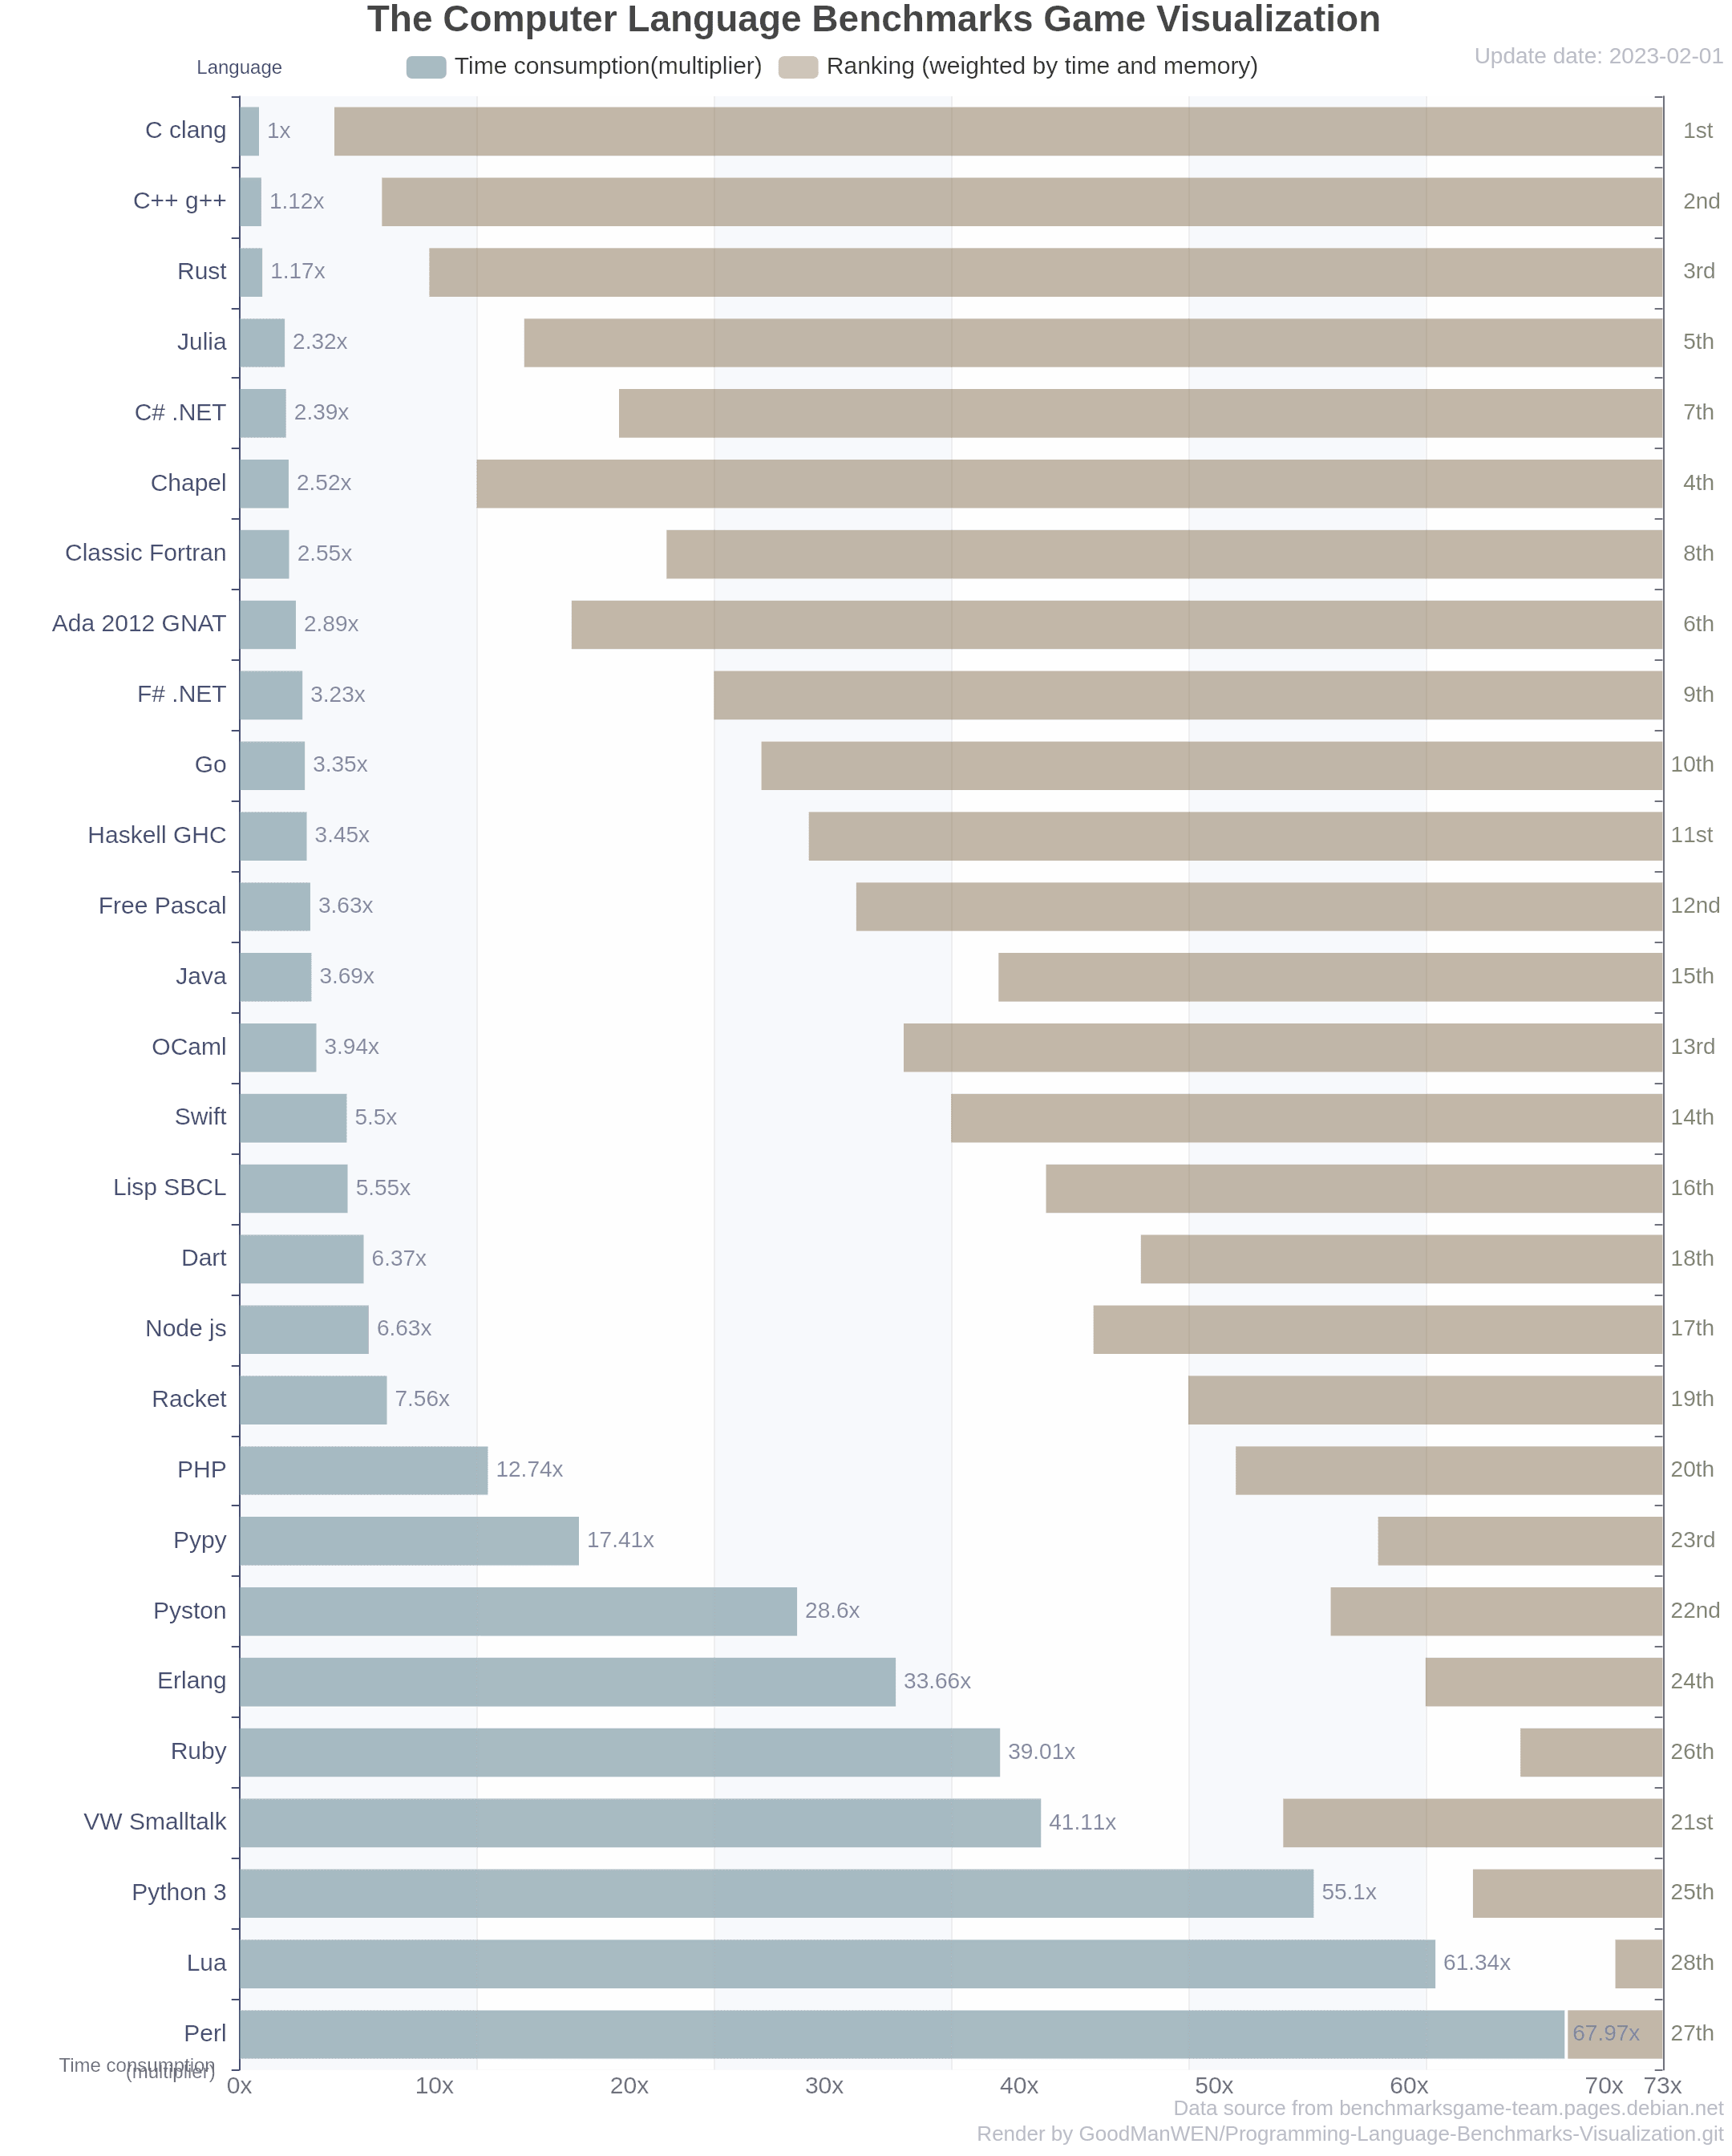
\includegraphics[width=\linewidth]{ranking}
				\caption{Programming Language Benchmarks Visualization \cite{actions2024GoodManWEN}}
			\end{figure}
		\end{minipage}
		\mypause
		\begin{minipage}{0.5\linewidth}
			\begin{itemize}
				\item Interpreted Language
				\item Global Interpreter Lock (GIL)
				\item Dynamic Typing
				\item Garbage Collection
			\end{itemize}
		\end{minipage}
	\end{frame}
	
	\subsection{Garbage Collector in Python}
	\begin{frame}{Garbage Collector in Python}
		\begin{itemize}
			\item \textbf{Garbage Collector (GC):} 
			A memory management tool that automatically deallocates unused objects in memory, preventing memory leaks.
			\item \textbf{How it works:}
			\begin{itemize}
				\item Python uses reference counting to keep track of objects.
				\item The GC handles cyclic references (e.g., objects referencing each other).
			\end{itemize}
			\item \textbf{\texttt{gc} module:}
			\begin{itemize}
				\item Provides an interface to the garbage collector.
				\item Functions:
				\begin{itemize}
					\item \texttt{gc.collect()}: Force a garbage collection.
					\item \texttt{gc.get\_stats()}: Get statistics on memory management.
					\item \texttt{gc.disable()}/\texttt{gc.enable()}: Turn GC off/on.
					\item \texttt{gc.garbage}: List of uncollectable objects.
				\end{itemize}
				\item Useful for debugging memory issues in Python applications.
			\end{itemize}
		\end{itemize}
	\end{frame}
	
	\begin{frame}{Comparison of Popular IDEs}
		\begin{adjustbox}{scale=.9}
		\begin{minipage}{1.11\linewidth}
		\begin{itemize}	
			\item \textbf{PyCharm:}
			\hfill\raisebox{-.2cm}{
\includegraphics[height=.7cm]{pycharm}}
			\begin{itemize}
				\item Best for professional Python development.
				\item Advanced debugging, intelligent code completion, and project management tools.
			\end{itemize}
			\item \textbf{VS Code:}
			\hfill\raisebox{-.2cm}{
\includegraphics[height=.7cm]{vscode}}
			\begin{itemize}
				\item Lightweight and highly customizable.
				\item Extensive extensions for Python, Git integration, and multiple language support.
				\item Built-in support for SSH for remote development.
			\end{itemize}
			\item \textbf{Spyder:}
			\hfill\raisebox{-.2cm}{
\includegraphics[height=.7cm]{spyder}}
			\begin{itemize}
				\item Designed for scientific computing and data analysis.
				\item Includes a variable viewer, similar to MATLAB's workspace.
				\item Seamlessly integrates with \texttt{NumPy}, \texttt{Pandas}, and \texttt{Matplotlib}.
			\end{itemize}
			\item \textbf{Jupyter Notebook:}
			\hfill\raisebox{-.2cm}{
\includegraphics[height=.7cm]{jupyter}}
			\begin{itemize}
				\item Ideal for interactive coding, data visualization, and educational purposes.
				\item Supports inline plots and markdown for creating documentation-rich notebooks.
			\end{itemize}
		\end{itemize}
		\end{minipage}
		\end{adjustbox}
	\end{frame}
	
	\begin{frame}{Popular Python Libraries for Scientific Computing}
		\textbf{Overview of Key Libraries}
		\begin{itemize}
			\item \textbf{NumPy:}
			\begin{itemize}
				\item Provides support for multi-dimensional arrays and matrices.
				\item Includes mathematical functions for efficient numerical computations.
				\item Serves as the foundation for many other libraries like SciPy and Pandas.
			\end{itemize}
			\item \textbf{SciPy:}
			\begin{itemize}
				\item Builds on NumPy to include advanced mathematical, scientific, and engineering functions.
				\item Offers modules for optimization, signal processing, linear algebra, and more.
			\end{itemize}
			\item \textbf{Pandas:}
			\begin{itemize}
				\item Focuses on data manipulation and analysis.
				\item Provides powerful tools for working with structured data, such as DataFrames.
				\item Ideal for handling missing data, merging datasets, and time-series analysis.
			\end{itemize}
		\end{itemize}
		

	\end{frame}
	
	
	\begin{frame}{Popular Python Libraries for Scientific Computing}
			\textbf{Why These Libraries Matter}
	\begin{itemize}
		\item Enable high-level, MATLAB-like functionality for numerical computations and data analysis.
		\item Combine performance with simplicity, making Python a powerful tool for scientific and engineering tasks.
		\item Offer extensive functionality while maintaining flexibility for a wide range of applications.
	\end{itemize}
		\end{frame}
		
		
	\begin{frame}{Popular Python Libraries for Data Visualization}
		\textbf{Overview of Key Libraries}
		\begin{itemize}
			\item \textbf{Matplotlib:}
			\begin{itemize}
				\item A versatile library for creating static, animated, and interactive visualizations.
				\item Supports a wide range of charts, including line plots, bar charts, scatter plots, histograms, pie charts, and more \supercite{matplotlibExamplesx2014}.
				\item Provides a MATLAB-like interface for ease of use.
			\end{itemize}
			\item \textbf{Seaborn:}
			\begin{itemize}
				\item Built on top of Matplotlib, focusing on statistical data visualization.
				\item Simplifies the creation of aesthetically pleasing and informative visualizations.
				\item Includes advanced plot types like heatmaps, pair plots, violin plots, and swarm plots.
				\item Provides built-in themes and color palettes for better design consistency.
			\end{itemize}
		\end{itemize}
	\end{frame}
	
		
		
		
		
		
		
		
		
		
	
	\begin{frame}[fragile]{Understanding Python Annotations}
		\textbf{What are Annotations?}
		\begin{itemize}
			\item Annotations are metadata added to function arguments and return values.
			\item They are used for documentation, type hinting, and static code analysis.
			\item Introduced in Python 3.0 and expanded in Python 3.5 with the \texttt{typing} module.
		\end{itemize}
		
%\begin{adjustbox}{scale=.9}
%	\begin{minipage}{1.11\linewidth}
		\begin{lstlisting}[caption=Using Annotations in Python]

def greet(name: str, age: int) -> str:
	"""
	Function to generate a greeting message.
	Args:
		name (str): The name of the person.
		age (int): The age of the person.
	Returns:
		str: A personalized greeting message.
	"""
	return f"Hello {name}, you are {age} years old!"
		\end{lstlisting}
%	\end{minipage}
%\end{adjustbox}
\end{frame}
	
	
	\begin{frame}{Using \texttt{typing} for Class Annotations}
		\textbf{Example: Annotating a Class with \texttt{typing}}
		\lstinputlisting[caption=Class Annotations with \texttt{typing}]{codes/examples/typing-example.py}
	
		
%		\textbf{Explanation:}
%		\begin{itemize}
%			\item \texttt{name: str} and \texttt{age: int} are basic type hints.
%			\item \texttt{skills: List[str]} specifies a list of strings.
%			\item \texttt{details: Optional[Dict[str, Union[str, int]]]} allows a dictionary with string keys and mixed string/integer values or \texttt{None}.
%			\item Annotations make the code easier to understand and suitable for static analysis.
%		\end{itemize}
	\end{frame}
	
	
	
	\begin{frame}[fragile]{Using \texttt{typeguard} for Runtime Type Checking}
		\begin{lstlisting}[language=Python, caption=Without \texttt{typechecked}]
def func(value: int) -> int:
	""" Multiplies the input value by 2. """
	return value * 2
# Example 1: Correct usage
print(func(5))  # Output: 10
# Example 2: Incorrect usage
print(func("5"))  # No error, Output: "55" (string concatenation)
		\end{lstlisting}
		
		\begin{lstlisting}[language=Python, caption=With \texttt{typechecked}]
from typeguard import typechecked

@typechecked
def func(value: int) -> int:
	""" Multiplies the input value by 2. """
	return value * 2
# Example 1: Correct usage
print(func(5))  # Output: 10
# Example 2: Incorrect usage
print(func("5"))  # TypeError: type of argument "value" must be int; got str instead
		\end{lstlisting}
	\end{frame}
	
	
	\begin{frame}{Introduction to \texttt{typeguard}}
		\textbf{Why Use \texttt{typeguard}\supercite{typeguardUserGuide}?}
		\begin{itemize}
			\item Ensures adherence to type annotations in dynamic typing environments.
			\item Useful for debugging and catching runtime type mismatches.
			\item Adds robustness to Python codebases, especially in large projects.
		\end{itemize}
		\mypause
		\textbf{Key Feature: \texttt{typechecked} Decorator \textcolor{red}{(?)}}
		\begin{itemize}
			\item The \texttt{@typechecked} decorator enforces type annotations on functions and methods.
			\item Validates:
			\begin{itemize}
				\item Function arguments.
				\item Return values.
			\end{itemize}
			\item Raises a \texttt{TypeError} if a mismatch is detected.
		\end{itemize}
	\end{frame}
	
	
	\begin{frame}{Understanding Decorators in Python}
		\textbf{What is a Decorator?}
		\begin{itemize}
			\item A decorator is a function that modifies the behavior of another function or method.
			\item They are used to extend or enhance functionality without modifying the original function's code.
			\item Commonly applied with the \texttt{@decorator\_name} syntax.
		\end{itemize}
		
		\textbf{How Does it Work?}
		\begin{itemize}
			\item A decorator takes a function as input and returns a new function.
			\item The new function wraps the original function, adding additional behavior.
		\end{itemize}
		
		\textbf{Why Use Decorators?}
		\begin{itemize}
			\item Code reusability and modularity.
			\item Useful for logging, validation, access control, etc.
			\item Simplifies and cleans up code by separating concerns.
		\end{itemize}
	\end{frame}
	
	
	\begin{frame}[fragile]{Example: Simple Decorator}
	\lstinputlisting[caption=Basic Decorator Example, lastline=12]{codes/examples/decorator-example.py}
	
	\mypause
	
	\lstinputlisting[firstline=18, lastline=22, firstnumber=13]{codes/examples/decorator-example.py}
	
	\mypause
	
	\lstinputlisting[firstline=13, lastline=17, frame=single,numbers=none]{codes/examples/decorator-example.py}
		
	\end{frame}
	
	\begin{frame}{\texttt{classmethod} and \texttt{staticmethod} as Decorators}
		\textbf{What are \texttt{classmethod} and \texttt{staticmethod}?}
		\begin{itemize}
			\item Both are \textbf{decorators} used to modify the behavior of methods in a class.
			\item They define how methods interact with the class or its instances:
			\begin{itemize}
				\item \texttt{classmethod:} Accesses and modifies class-level data.
				\item \texttt{staticmethod:} Behaves like a regular function but is logically grouped within the class.
			\end{itemize}
		\end{itemize}
	\end{frame}
		
	\begin{frame}[fragile]{Example Code:}
		\lstinputlisting[language=Python, caption=Using \texttt{classmethod} and \texttt{staticmethod}]{codes/examples/classmethods.py}
	\end{frame}
	
	
	\begin{frame}{\texttt{property} Decorator: Getter and Setter}
		\textbf{What is the \texttt{property} Decorator?}
		\begin{itemize}
			\item \texttt{property} is a built-in decorator in Python used to create managed attributes.
			\item It allows defining a method as a getter and optionally as a setter or deleter.
			\item Enables encapsulation by controlling access to an attribute.
		\end{itemize}
	\end{frame}
	
	
	\begin{frame}[fragile]{Example Code:}
		\lstinputlisting[language=Python, caption=Using \texttt{property} with Getter and Setter]{codes/examples/property-getter-setter.py}
	\end{frame}
	
	
	
	
	
	
	\begin{frame}[allowframebreaks]
		\frametitle{References}
		\printbibliography
	\end{frame}
	
	%----------------------------------------------------------------------------------------
	
\end{document} 

